
\marginpar{\href{https://youtu.be/EObHWIEKGjA}{Video}} Reading: Finish Chapter 2

\subsection{Independent Random Events}

\marginpar{(8m)}

\begin{align*}
p_{X,Y,Z}(x,y,z)=p_X(x)p_{Y|X}(y|x)p_{Z|X,Y}(z|x,y)
\end{align*}

Random variables X,Y,Z are independent if:
\begin{align*}
p_{X,Y,Z}(x,y,z)=p_X(x)p_{Y}(y)p_{Z}(z)
\end{align*}

\begin{figure}[h]
\centering
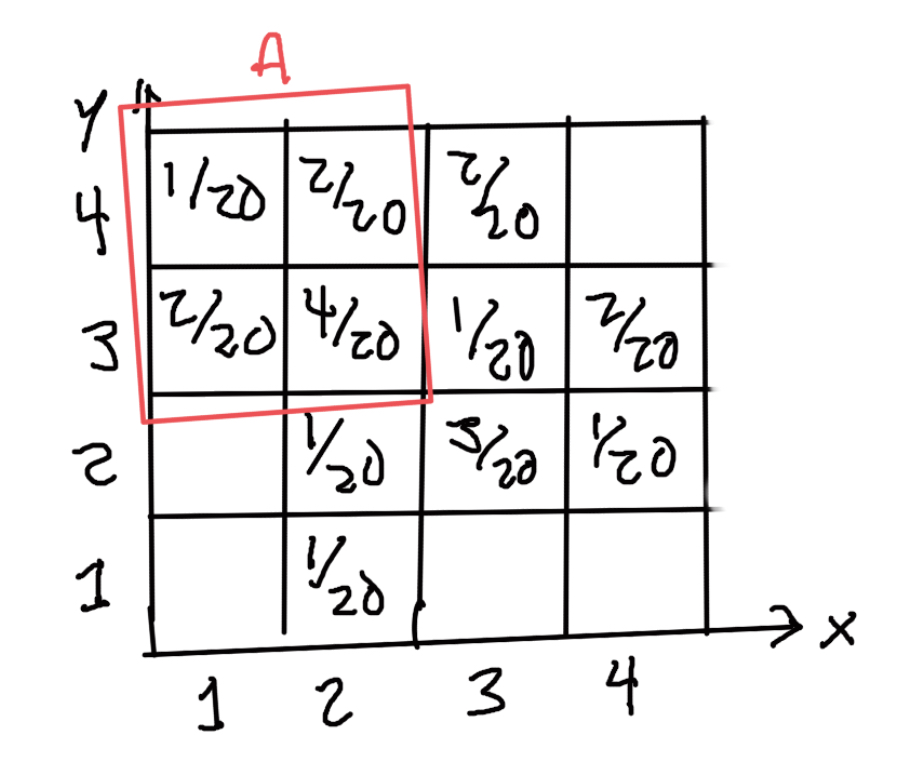
\includegraphics[width=6cm, height=4cm]{images/L07/IMG_1544.jpeg}
\caption{Joint PMFs}
\end{figure}

\begin{figure}[h]
\centering
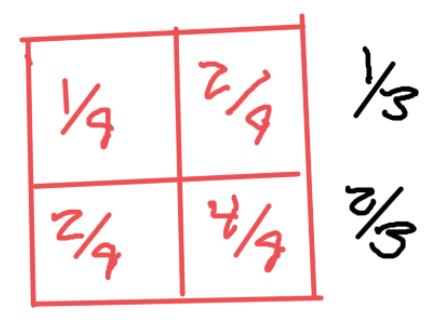
\includegraphics[width=5cm, height=4cm]{images/L07/IMG_1545.jpeg}
\caption{Joint PMFs}
\end{figure}

\marginpar{(19m)}

\marginpar{(28m)}

\subsection{Binomial Mean and Variance}
\marginpar{(32m)}

\subsection{Hat Problem}

\marginpar{(39m)}

\begin{figure}[h]
\centering
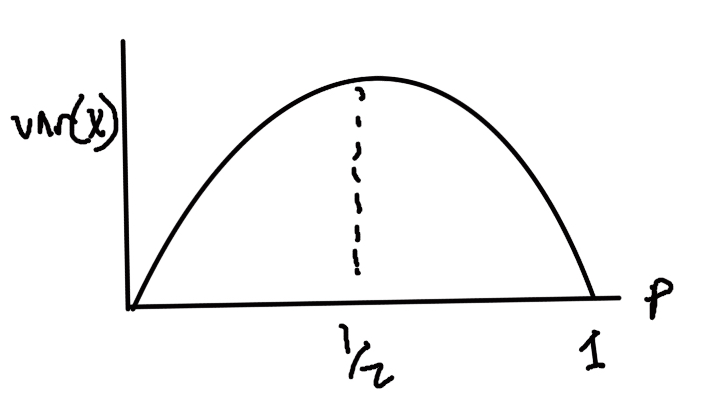
\includegraphics[width=5cm, height=4cm]{images/L07/bin_hat_problem.jpeg}
\caption{Hat Problem}
\end{figure}

\marginpar{(43:20)}

\begin{align*}
var(X) = E[X^2] - (E[X])^2
\end{align*}

$E[X^2]=2$

$var(X)=2-1=1$